%!TEX root = thesis.tex


\pagenumbering{arabic}

\chapter{Introduction}
\label{chap:Introduction}

\section{Background and Definitions}
This thesis studies the application of sums of squares to combinatorial optimization. 
In this section, we give a description of the general area of combinatorial optimization and sums of squares in particular.
We introduce many of the concepts which will be used in the following chapters. 
In the remainder of the introduction, we give an extended abstract of each chapter.

\subsection{Combinatorial Optimization}
Combinatorial optimization is the study of problems consisting of optimizing a function over a discrete set. 
Applications are common in computer science, mathematics, and operations research.
For example, the goal of the traveling salesman problem is to find a minimum-cost tour among a set of cities.
The goal of the shortest path problem is to find a shortest-distance path between two nodes in a graph.
And the goal of the assignment problem is to assign workers to jobs while minimizing the total wages paid. 

In each of the above problems, we minimize a linear function over a finite set.
For instance, in the traveling salesman problem, we want to find the minimum of $f(T) = \sum_{e \in E} c_ex_e$ over all tours $T$.
Here, a tour is represented by a 0/1 vector $x \in \mathbb{R}^{n \choose 2}$, with $x_e = 1$ if and only if the edge $e$ is part of $T$.
The weights $c_e$ are part of the problem data and represent the cost to travel along edge $e$.

A common approach is to rewrite this as a linear program. 
The problem is naturally an integer linear program, as we can replace the constraints $x_e \in \{0,1\}$ by $x_e \in \mathbb{Z}$, $0 \le x_e \le 1$, and encode the fact that $T$ is a tour using other linear constraints.
But since we optimizea linear function, the optimum is unchanged if we instead consider the convex hull $\textup{TSP}(G)$ of all tours.
This is a natural object to study without referring to a specific set $(c_e)$ of weights, since changing the weights is equivalent to optimizing in a different direction over $\textup{TSP}(G)$.

To construct this convex hull in general, consider a problem where we optimize over some feasible collection $\mathcal{C}$ of subsets of a fixed set $X$.
For instance, in the TSP we let $\mathcal{C}$ be the collection of all tours; here $X$ is the set of edges.
In the shortest-path problem we consider $\mathcal{C}$ to be the collection of all paths from a fixed $x \to y$; again $X$ is the set of edges.
A non-graph example is the knapsack problem, where $\mathcal{C}$ is the set of subsets of $X = \{1, \ldots, n\}$ satisfying a capacity constraint.
In general, we will assume that $X = \{1, \ldots, n\}$ for some $n$; this can always be accomplished by enumerating $X$.
For each $C \in \mathcal{C}$, define its characteristic vector $\chi_C \in \{0,1\}^n$, where for $1 \le i \le n$, $(\chi_C)_i = 1$ if and only if $i \in C$.
Then define the polytope $P(\mathcal{C}) = \conv \{\chi_C: C \in \mathcal{C}\}$.
If we can optimize in polynomial time over $P(\mathcal{C})$ in any direction, we have solved the problem associated to $\mathcal{C}$.

Of course, many combinatorial optimization problems often end up being NP-complete or harder. 
That is, we are unlikely to ever find efficient algorithms to solve them exactly.
And in some cases where the abstract mathematical problem does have an efficient algorithm, real-world constraints can make it intractable. 
For instance, when assigning medical students to residencies, the constraint that married pairs of students live in the same city makes the problem NP-complete.
Therefore, much research has focused on developing methods to solve these problems approximately. 
Using various methods, we can construct a relaxation $P'(\mathcal{C})$ to $ P(\mathcal{C})$ and try to show that the gap between them is not very large.
In the next section, we describe one such method based on sums of squares.

\subsection{Sums of Squares and the Theta Body}
Consider for the moment unconstrained polynomial optimization problems on $\RR^n$. 
That  is, we are given a polynomial $f$ in $n$ real variables, and must find the global minimum value $f_{\min}$. 
It turns out that optimization is closely related to checking nonnegativity.
If we can find the global minimum of a polynomial $f$, we can certainly check if $f$ is nonnegative everywhere by checking if its minimum $f_{\min} \ge 0$.
Conversely, if we can check whether polynomials are nonnegative, we can compute $f_{\min}$: observe that $f_{\min} = \max \{r: f(x) - r \ge 0\}$. 
We can solve the latter problem by sampling different $r$ (e.g. with binary search) and for each $r$ checking whether $f - r$ is nonnegative.

Checking arbitrary polynomials for nonnegativity is NP-hard, so we seek an approximation.
Note that if we can write $f(x)$ as a sum of squares, then it is certainly nonnegative. 
Therefore, we can define the relaxation $f_{\textup{sos}} = \max \{r: f(x) - r \textup{ is a sum of squares}\}$.
We have that $f_{\min} \ge f_{\textup{sos}}$, so this is a lower bound on the minimum. 
This idea is discussed at more length in \cite{sostools} and \cite{lasserre}. 

So far, this only makes sense for polynomials on $\mathbb{R}^n$.
We will define a notion of sums of squares that is applicable to combinatorial optimization problems.
This definition originated with Lovasz \cite{lovasz} and was used to produce an approximation to the stable set problem.
It was generalized to arbitrary problems by Gouveia, Parrilo, and Thomas \cite{gpt}.

As in section 1.1.1, consider a collection $\mathcal{C}$ of subsets of $\{1, \ldots, n\}$. 
Let $V = \{\chi_C: C \in \mathcal{C}\}$.
$V$ is a finite set, and therefore an {\em algebraic variety}.
That is, it is the set of solutions of a finite list of polynomials.
The {\em ideal} $I$ of $V$ is defined to be the set of all polynomials vanishing on $V$.
We can define an equivalence relation on polynomials, denoted $f \equiv g \mod I$, if and only if $f - g \in I$.
It turns out that $f \equiv g \mod I$ if and only if $f(x) = g(x)$ for each $x \in V$.
For a polynomial $f$ and an integer $k$, we say $f$ is {\em $k$-sos mod $I$} if we can write $f \equiv \sum_i g_i^2 \mod I$ for some polynomials $g_i$ with degree at most $k$.
Now define the $k$th {\em theta body} of $I$, $\textup{TH}_k(I)$, to be the intersection of all affine linear functions $f$ which are $k$-sos mod $I$. 
This defines a relaxation of the convex hull of $V$: $\conv(V) \subseteq \textup{TH}_k(I)$ for each $k$, with the approximation improving as $k$ increases.
We can optimize over $\textup{TH}_k(I)$ in polynomial time for fixed $k$ using semidefinite programming, so this provides an efficient relaxation to $P(\mathcal{C}) = \conv(V)$.

\section{A Semidefinite Approach to the $K_\MakeLowercase{i}$-Cover Problem}
Chapter 2 is taken from a paper coauthored with Jo\~ao Gouveia and submitted to \emph{Operations Research Letters}. 

\subsection{Problem Description}

The {\em $K_i$-cover problem} is a generalization of the stable set problem discussed in Chapter 1.1. 
A graph $G = (V,E)$ is given. 
For any $k$, a $k$-clique in $G$, denoted $K_i$, is a collection of $k$ nodes, each pair of which is connected by an edge in $E$.
We define a covering relation where an $i$-clique $H_1$ is covered by an $(i-1)$-clique $H_2$ if $H_1 \supseteq H_2$; i.e., if $H_2$ is a subgraph of $H_1$. 
A $K_i$-cover in $G$ is a collection $\mathcal{F}$ of $(i-1)$-cliques in $G$ such that each $i$-clique in $G$ is covered by some element of $\mathcal{F}$. 
The $K_i$-cover problem is to find such a collection $\mathcal{F}$ of smallest size.
In the graph $G$ in Figure \ref{K5}, a $K_4$-cover is given by $\{012,034,023\}$.

\begin{figure}[htd]
	\centering
	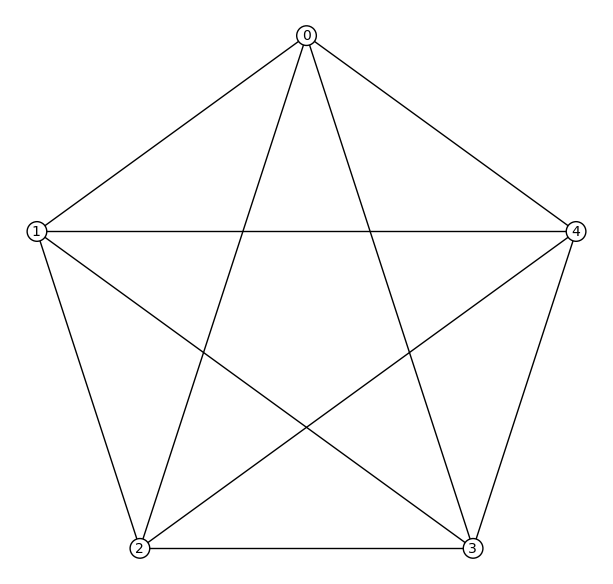
\includegraphics[width=.4\textwidth,natwidth=613,natheight=584]{K5.png}
	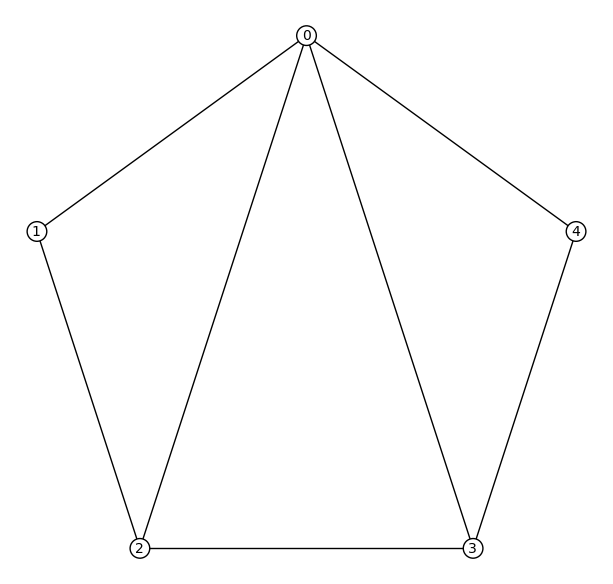
\includegraphics[width=.4\textwidth,natwidth=613,natheight=584]{K4cover.png}
	\caption{A graph with 5 copies of $K_4$: 0123,0124,0134,0234,1234; along with a possible $K_4$-cover.}
	\label{K5}
\end{figure}

When $i=2$, this is the \emph{vertex cover problem} - to find the smallest set $\mathcal{F}$ of vertices such that each edge is covered by a vertex in $\mathcal{F}$. 
To make the connection to the stable set problem, note that $\mathcal{F} \subseteq V$ is a vertex cover if and only if $V \setminus \mathcal{F}$ is a stable set.
Therefore, the problems are essentially equivalent.
In fact, the polytopes defined by these problems as in section 1.1 are congruent via the transformation $x_j \mapsto 1-x_j$ in each coordinate.

\subsection{Background}

The stable set and vertex cover problems have been studied in many contexts. 
The $K_i$-cover generalization was first studied in Conforti et al \cite{conforti}, wherein the associated polytope $P_i(G)$ was considered and several families of facets identified. 
As in Section 1.1, $P_i(G) \subseteq \mathbb{R}^N$ is the convex hull of characteristic vectors of $K_i$-covers, where $N$ is the number of $K_{i-1}$s in $G$. 
Conforti et al provided polynomial-time {\em separation oracles} for many of these families of facets. 
A separation oracle for a family $\mathcal{F}$ of facets is a decision procedure which takes a point $x$ and decides whether $x$ satisfies each facet $F \in \mathcal{F}$, or whether $x$ lies outside some facet $F \in \mathcal{F}$.
Since a typical family $\mathcal{F}$ will contain exponentially many elements, it is not possible in general to enumerate the $F \in \mathcal{F}$ and check them one by one, making such an oracle a nontrivial result.

Conforti et al left open the existence of oracles for several families of facets, including the family associated with the {\em $K_i$-$p$-holes}. 
A graph $H$ is a $K_i$-$p$-hole if it contains $p$ copies of $K_i$ arranged in a cycle, with neighboring $K_i$ sharing a common $K_{i-1}$. 
This does not determine $H$ up to isomorphism; see Figure 2 for three nonisomorpic $K_3$-9-holes.
To understand the facet inequality associated to a $K_i$-$p$-hole, consider the graphs in Figure 2. 
To construct a $K_3$-cover of minimum size, we need to pick an edge from each $K_3$. 
We can pick four edges to eliminate eight $K_3$s, but we still need a fifth to pick up the last $K_3$. 
Therefore, $\sum_{e \subseteq H} x_e \ge 5$ is valid on the polytope $P_3(G)$ for any graph $G$ containing $H$ as a subgraph. 
The inequality for general $K_i$-$p$-holes is derived from a similar argument, and is given by $\sum_{e \subseteq H} x_e \ge \lceil \frac{p}{2} \rceil$.
It defines a facet of $P_i(G)$ for $i \ge 3$ and odd $p$.

\begin{figure}[htd]
	\centering
	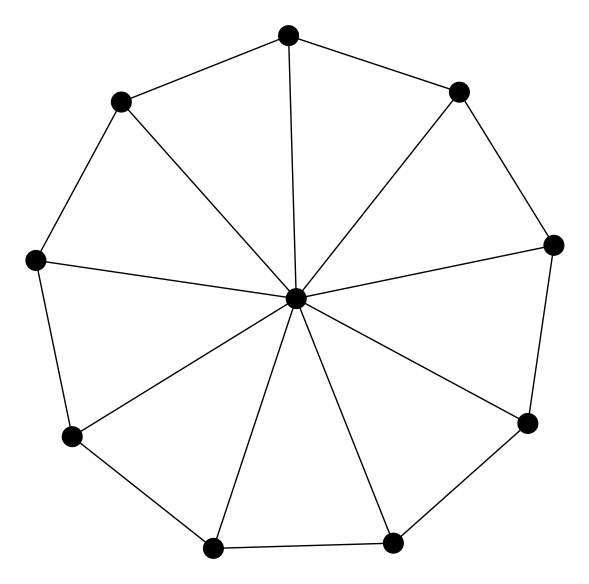
\includegraphics[width=.3\textwidth,natwidth=589,natheight=584]{9holeA.png}
	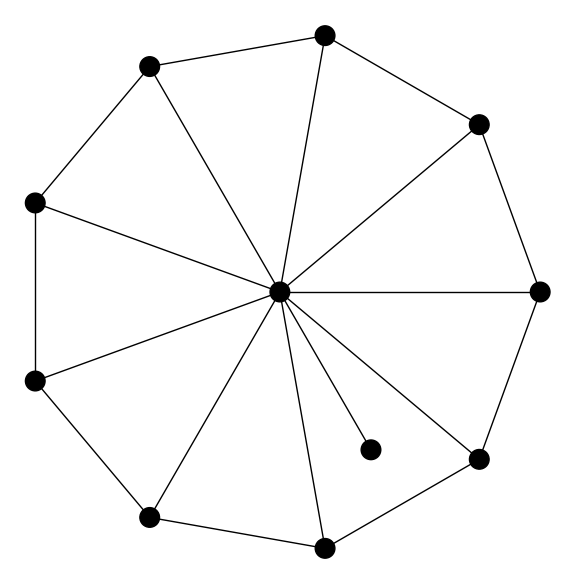
\includegraphics[width=.3\textwidth,natwidth=575,natheight=584]{9holeB.png}
	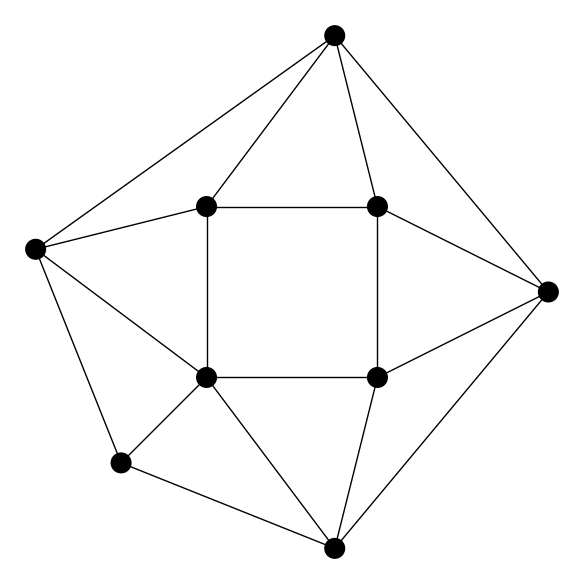
\includegraphics[width=.3\textwidth,natwidth=584,natheight=584]{9holeC.png}
	\caption{Three non-isomorphic $K_3$-9-holes.}
	\label{9holeintro}
\end{figure}

\subsection{Results}
\begin{itemize}
\item We show that the family of facets corresponding to $K_i$-$p$-holes is valid on the theta body $\textup{TH}_{\lceil i/2\rceil }(G)$.
Therefore, for fixed $i$, we have a polynomial-time algorithm to optimize over a relaxation at least as tight as this family. 
To show that the $K_i$-$p$-hole facets are valid on $\textup{TH}_{\lceil i/2\rceil}(G)$, we choose a set of  polynomials which are idempotent mod $I$, and whose sum is the facet-defining inequality.
\item We consider the triangle free problem, the special case $i=3$ of the $K_i$-free problem. We show that $P_3(K_n) \subsetneq \textup{TH}_{k}(K_n)$ for $k < n/2$.
That is, it takes at least $n/2$ steps for the theta body heirarchy to converge to the triangle free polytope for $K_n$, and therefore this heirarchy does not give a polynomial-time algorithm for the triangle free problem.
We show this by observing that the cut polytope and triangle free polytope of $K_n$ share a facet, and apply a result of Laurent \cite{moniquestuff} that the theta heirarchy takes at least $n/2$ steps to reach this facet.
\item We show that there is an {\em integrality gap} of $1/2$ for the triangle cover's second theta relaxation. 
That is, if we optimize in the all-1 direction in the triangle cover problem, we have $\min \{1 \cdot x: x \in \textup{TH}_2(G) \} \ge \frac{1}{2} \min \{1 \cdot x: x \in P_3(G)\}$ for all $G$. 
We prove this by applying a result of Krivelevich \cite{krivelevich} on a fractional relaxation of the same problem, and proving that $\textup{TH}_2(G)$ is contained in this fractional relaxation.
\end{itemize}
\subsection{Comments}
We don't fully address the question raised in Conforti of whether there is a polynomial time separation oracle for the family $\mathcal{F}$ of $K_i$-$p$-hole facets.
We show that the facets are valid on $\textup{TH}_{\lceil i/2\rceil}(G)$, and that we can check membership of $\textup{TH}_{\lceil i/2 \rceil}$ in polynomial time. 
However, this does not give a separation oracle for $\mathcal{F}$.
Indeed, let $Q$ be the body defined as the intersection of all $F \in \mathcal{F}$.
We have $P_i(G) \subseteq \textup{TH}_{\lceil i/2\rceil}(G) \subseteq Q$, so in terms of an approximation to $P_i(G)$, the theta body is tighter, and we can optimize over it in polynomial time (for fixed $i$).
However, this doesn't allow us to optimize over exactly $Q$ in polynomial time.
In fact, for $i=2$, the stable set case, we have a similar phenomenon: $\textup{STAB}(G) \subseteq \textup{TH}(G) \subseteq \textup{QSTAB}(G)$. 
Here STAB is the convex hull of stable sets in $G$ and QSTAB is the LP relaxation given by clique inequalities.
In this case it is NP-hard to optimize over either STAB or QSTAB, while TH can be optimized over in polynomial time.


Conforti et al \cite{conforti} found additional facets of $P_i(G)$, associated to other subgraphs of $G$, for which no separation oracle is currently known. 
We checked numerically and found that they did not appear to be valid on $\textup{TH}_{\lceil i/2\rceil}(G)$, but they may be valid on higher theta bodies.




\section{Sums of Squares on the Unit Hypercube}

Extended abstract of the cube paper goes here.

\section{Flag Algebras and Sums of Squares}

Extended abstract of the flag algebras paper goes here.

\section{The Representation Theory of Matchings}

Extended abstract of the matchings paper goes here.

\section{A Note on Notation}
The following chapters were published as separate papers, and in some cases refer to different aspects of the same or related problems. 
As such, the chapters use different notation to fit the topic at hand, so the same object may have different names in different chapters.
